\section{Experimental Setup}
\label{sec:experiments}

\paragraph{Research questions and hypotheses.}
\textbf{RQ1} (compute-matched): does MCTS exceed cheaper search at equal token
budget? \textbf{RQ2} (policy): how does the marginal search gain $\gain$ depend on
policy strength $\polacc$? \textbf{RQ3} (reward): is the bottleneck the policy or
the reward? \textbf{RQ4} (search space): taxonomy vs.\ reasoning search?
The corresponding hypotheses are
\textbf{H1} $\Acc_{\mctstax}(\budget) - \Acc_{\text{SC}}(\budget) \le \epsilon$ for
weak policies;
\textbf{H2} $\gain$ increases in $\polacc$ with a threshold $\alpha^\star$ below
which $\gain \le 0$;
\textbf{H3} switching self-eval$\to$judge moves leaf accuracy by $\ll$ the gain
from a stronger policy;
\textbf{H4} reasoning search beats taxonomy search for weak policies.

\subsection{Datasets and Splits}
All examples come from BigVul \citep{fan2020bigvul}: vulnerability-fixing
commits in C/C++ projects rendered as unified diffs with the commit message
(Appendix~\ref{app:data}). The dev set ($n{=}50$, prompt iteration only) is
drawn from BigVul's validation split and the evaluation pool ($n{=}500$,
stratified by CWE) from its test split, so prompt development cannot overfit
the evaluation data. The CWE trees (operational and full-depth,
\S\ref{sec:problem}) are built from MITRE relationships and released with
SHA-256 hashes. A temporal split by CVE year is reported as a robustness check
(\S\ref{sec:analysis}).

\paragraph{Pretraining-leakage control.}
LLMs may have seen public CVEs during pretraining; BigVul's CVEs (2006--2019)
all predate every policy's training cutoff, so a post-cutoff ``fair slice'' is
not constructible from this corpus. We instead verify that conclusions are
stable across CVE years (\S\ref{sec:analysis}) and note that leakage shifts
absolute accuracies, not the within-budget strategy comparisons that are the
object of study --- all strategies share the same policy and examples.

Data statistics (sources, splits, per-category composition, tree hashes) are
given in Appendix~\ref{app:data}.

\subsection{Strategies and Models}
The seven strategies of \S\ref{sec:method} all use the same policy and prompt.
We use five policies spanning the strength axis required for H2: four
cheap-tier (GPT-4.1-nano, Gemini-2.5-Flash-Lite, DeepSeek-V3.1 --- open-weight
--- and Claude-Haiku-4.5) plus a premium policy (Claude-Sonnet-4.6) on a
reduced sample for the strong end. The external judge is a model stronger than
the policy it judges (Claude-Haiku-4.5 judging GPT-4.1-nano); each
$(\policy,\text{judge})$ pair is logged.

\subsection{Compute-Matched Protocol}
We measure $\mathrm{tok}_X(c)$ per knob value (Table~\ref{tab:a2}), giving a
budget grid that spans $1\times$--$10\times$ a single greedy pass, and compare
strategies \emph{only} at comparable measured budgets --- including across
search spaces, where we sweep the $\mctsreas$ iteration knob down until its
budget falls below $\mctstax$'s. We additionally analyze sequential depth and
wall-clock latency (\S\ref{sec:analysis}): self-consistency parallelizes
trivially, MCTS does not --- a practically important asymmetry.

\subsection{Metrics and Statistics}
Primary: leaf accuracy, category (level-0) accuracy, hierarchical-$F_1$ on path
edges \citep{kosmopoulos2015evaluation}, and the accuracy-vs-budget curve
$\Acc_X(\budget)$; secondary: tokens/sample and sequential depth. Stochastic
configurations use $5$ seeds on the weak-policy grid and $3$ on the other
policies (deterministic strategies run once); we report mean $\pm$ std across
seeds, and strategy comparisons at comparable budgets use paired McNemar.

\section{Results}
\label{sec:results}

\subsection{RQ1: Search vs.\ Compute (the headline)}

Table~\ref{tab:matched} reports the compute-matched comparison on a \emph{weak}
policy (GPT-4.1-nano) and a \emph{strong} policy (Claude-Haiku-4.5), on BigVul
examples (diff$+$commit-message input, $7$-category code-aligned tree), comparing
greedy, self-consistency, and $\mctstax$ at a token budget where the latter two
spend roughly equally within each policy (nano $n{=}300$/$5$ seeds, Haiku
$n{=}150$/$3$ seeds; the full pairwise significance matrix is in
Appendix~\ref{app:extra}).

\begin{table}[t]
\centering
\small
\begin{tabular}{l cc cc}
\toprule
 & \multicolumn{2}{c}{nano (weak)} & \multicolumn{2}{c}{Haiku (strong)} \\
\cmidrule(lr){2-3}\cmidrule(lr){4-5}
Strategy & Leaf & Cat.\ & Leaf & Cat.\ \\
\midrule
Greedy (no search)         & $14.7$ & $28.7$ & $24.7$ & $46.7$ \\
Self-Consistency ($N{=}8$) & $16.5$ & $31.5$ & $24.0$ & $46.7$ \\
$\mctstax$ ($I{=}16$)      & $\mathbf{22.9}$ & $\mathbf{39.5}$ & $\mathbf{26.6}$ & $44.4$ \\
\midrule
$\gain$ ($\mctstax$ $-$ greedy) & $+8.2$ & $+10.8$ & $+1.9$ & $-2.3$ \\
\bottomrule
\end{tabular}
\caption{Compute-matched test-time search (accuracy \%), weak vs.\ strong policy
(nano $n{=}300$/$5$ seeds; Haiku $n{=}150$/$3$ seeds, greedy and SC deterministic
or $1$ seed). At equal budget, $\mctstax$ lifts the
weak policy by $+8.2$ (leaf) / $+10.8$ (category) points, but the strong policy by
only $+1.9$ / $-2.3$. Self-consistency helps neither. The marginal search gain
$\gain$ \emph{shrinks} as policy strength grows.}
\label{tab:matched}
\end{table}

\textbf{Finding.} (i) On the weak policy, at matched compute, reward-guided tree
search clearly beats both no-search and sampling-without-reward: $\mctstax$ reaches
$22.9\%$ leaf accuracy versus $16.5\%$ (self-consistency) and $14.7\%$ (greedy);
across-seed std is $\le 1.0$. Both gaps are significant by paired McNemar
($\mctstax$ vs.\ greedy $p{=}8\!\times\!10^{-6}$; vs.\ self-consistency
$p{=}2\!\times\!10^{-3}$, $n{=}300$). Self-consistency---majority vote over
independent samples, ignoring the reward---captures only $+1.8$ points, whereas
MCTS, using the same self-evaluation reward to \emph{steer} the search, captures
$+8.2$. Best-of-$N$ ($N{=}8$), which keeps the reward but drops the tree
(independent samples, return the highest-scoring path), lands in between: $+6.4$
leaf points at a \emph{larger} budget ($15.8$k vs.\ $10.7$k tokens). Reading the
three together: the reward signal alone recovers most of the sampling family's
gap to tree search, and the tree adds the rest while spending less. (ii) On the strong policy the same search yields little ($+1.9$ leaf) to
nothing ($-2.3$ category): the strong policy is already near the signal available
in the input, so reward-guided exploration mostly reconfirms or drifts. Test-time
search here acts as a \emph{compensator for weak policies}, not a universal
improvement.

\subsection{RQ2: Search Gain vs.\ Policy Strength}
Across five policy points the marginal search gain $\gain$ of $\mctstax$ over
greedy (category accuracy) \emph{decreases monotonically} with policy strength
$\polacc$:
%
\begin{center}\small
\begin{tabular}{lccccc}
\toprule
Policy & Gemini-FL & nano & DeepSeek & Haiku & Sonnet \\
$\polacc$ (greedy cat.) & $0.28$ & $0.29$ & $0.37$ & $0.47$ & $0.48$ \\
\midrule
$\gain$ ($\mctstax$, cat.) & $+6.7$ & $+10.8$ & $+2.0$ & $-2.3$ & $+1.7$ \\
$\gain$ ($\mctsreas$, cat.) & $+14.2$ & $+19.4$ & $+8.2$ & $-3.8$ & $+2.5$ \\
\bottomrule
\end{tabular}
\end{center}
%
The taxonomy-search gain falls from $+7$--$11$ points at the weak end
($\polacc \approx 0.28$, two independent policies) to $\approx 0 \pm 3$ at the
strong end (Haiku $-2.3$, Sonnet $+1.7$); the reasoning-search gain starts far
higher ($+14$--$19$) and collapses onto the same near-zero band ($-3.8$ /
$+2.5$). At the strong end the residual gains are within noise of zero at this scale.

This \textbf{contradicts our pre-registered H2}, which anticipated that gain would
\emph{increase} with $\polacc$ (a threshold $\alpha^\star$ below which search
fails). The data show the opposite ordering: search is most valuable exactly where
the policy is weakest, and vanishes as the policy approaches the accuracy ceiling
imposed by the task/labels (\S\ref{sec:analysis}). We therefore revise the claim:
test-time search trades compute for accuracy on under-powered policies, and offers
diminishing-to-negative returns on strong ones.

One nuance: on the mid-strength policy (DeepSeek), plain self-consistency
($N{=}8$: $28.2$ leaf) actually edges out $\mctstax$ ($25.3$) while both trail
$\mctsreas$ ($27.8$ leaf, $44.9$ category) --- so the pre-registered H1
($\mctstax$ within $\epsilon$ of self-consistency at matched budget) fails for
the weak policy but roughly holds mid-scale. The ordering that is stable across
all three policies is the search-space one (RQ4).

\emph{(nano $n{=}300$/$5$ seeds; DeepSeek and Haiku $n{=}130$--$150$/$3$ seeds;
Sonnet $n{=}120$/$1$ seed; all evaluation sets are prefixes of one fixed,
shuffled example file, and greedy is deterministic.)}

\subsection{RQ3: Is the Reward the Bottleneck?}
If reward fidelity limited MCTS, replacing the policy's self-evaluation with a
stronger external judge (Claude-Haiku-4.5, the strong policy of RQ1, judging the
weak nano policy) should help. On matched examples ($n{=}300$, $3$ seeds):
for $\mctstax$ ($I{=}16$) the judge changes nothing --- $22.8 \pm 0.5$ leaf
accuracy vs.\ $22.9 \pm 0.1$ with self-evaluation --- while costing $71\%$ more
tokens ($18.3$k vs.\ $10.7$k). For $\mctsreas$ ($I{=}8$) the judge yields a small
gain ($35.4 \pm 0.6$ vs.\ $33.9 \pm 0.3$) at $27\%$ more tokens; but self-eval
$\mctsreas$ at $I{=}2$ already reaches $34.8 \pm 0.4$ at less than a \emph{third}
of the judge configuration's budget, so the gain does not survive compute
matching.

\textbf{Finding.} Upgrading reward fidelity does not move taxonomy search at all
--- its early-commitment pathology is structural, and no reward source can fix a
search-space problem --- and buys, on reasoning search, less than its extra
tokens are worth elsewhere. The reward source is therefore not the binding
constraint; the policy and the search space are (consistent with RQ2 and RQ4).
A reward-calibration analysis (AUROC of rollout reward vs.\ correctness for
both reward sources) corroborates this reading in \S\ref{sec:analysis}.

\subsection{RQ4: Taxonomy vs.\ Reasoning Search}
We compare MCTS over the taxonomy ($\mctstax$, committing level-by-level) against
MCTS over a free-form reasoning trajectory ($\mctsreas$, which reasons and then
commits directly to a leaf), at a comparable budget on the weak policy
(Table~\ref{tab:m4m5}, $n{=}150$).

\begin{table}[t]
\centering
\small
\begin{tabular}{l cc cc}
\toprule
 & \multicolumn{2}{c}{nano (weak)} & \multicolumn{2}{c}{Haiku (strong)} \\
\cmidrule(lr){2-3}\cmidrule(lr){4-5}
Strategy & Leaf & Cat.\ & Leaf & Cat.\ \\
\midrule
Greedy                & $14.7$ & $28.7$ & $24.7$ & $46.7$ \\
$\mctstax$ ($I{=}16$) & $22.9$ & $39.5$ & $26.6$ & $44.4$ \\
$\mctsreas$ ($I{=}8$) & $\mathbf{33.9}$ & $\mathbf{48.1}$ & $\mathbf{28.4}$ & $42.9$ \\
\bottomrule
\end{tabular}
\caption{Taxonomy vs.\ reasoning search (accuracy \%; nano $n{=}300$/$5$ seeds,
Haiku $n{=}150$/$3$ seeds). Reasoning search beats taxonomy search on \emph{both}
policies; the margin is large for the weak policy ($+11$ leaf) and modest for the
strong one ($+1.8$).}
\label{tab:m4m5}
\end{table}

\textbf{Finding.} Reasoning-trajectory search dominates taxonomy search on
\emph{both} policies (weak: $33.9$ vs.\ $22.9$ leaf, $+11$, paired McNemar
$p{=}3.2\!\times\!10^{-4}$, $n{=}300$; strong: $28.4$ vs.\ $26.6$, $+1.8$), with
the advantage shrinking as the policy strengthens (cf.\ RQ2). On the strong
policy it trades a small category drop ($42.9$ vs.\ greedy $46.7$) for a leaf
gain, reaching finer leaves at the cost of occasionally landing in a neighbouring
category. On the premium policy (Sonnet, $n{=}120$, $1$ seed) the ordering
\emph{reverses} on leaf accuracy ($31.7$ vs.\ $35.0$ for $\mctstax$): a policy
that already reasons well in a single pass gains nothing from an external
reasoning scaffold, while the taxonomy structure still adds a little fine-grained
discrimination. The search-space advantage, like the search gain itself, is a
property of \emph{weak-to-mid} policies.

\paragraph{Strict budget matching.}
Sweeping $\mctsreas$ over $I \in \{2,4,6,8\}$ ($n{=}300$, $5$ seeds,
Figure~\ref{fig:budget}) shows its accuracy is \emph{flat in the iteration count}:
$I{=}2$, at $5.3$k tokens/example --- \emph{half} of $\mctstax$'s $10.7$k budget
--- already reaches $34.8\%$ leaf / $50.4\%$ category accuracy, slightly
\emph{above} $I{=}8$ ($33.9$ / $48.1$). The dominance over taxonomy search
therefore survives strict budget matching with room to spare ($\mctsreas$ at
$I{=}2$ vs.\ $\mctstax$ at $I{=}16$: paired McNemar $p{=}8.7\!\times\!10^{-5}$;
vs.\ greedy: $p{=}4.4\!\times\!10^{-10}$). The flatness is itself informative:
nearly all of $\mctsreas$'s gain comes from its \emph{representation} --- reason
first, commit to a leaf directly --- rather than from accumulating search
statistics; we return to this in \S\ref{sec:analysis}.

The mechanism is the cascade (Proposition~\ref{prop:cascade}): $\mctstax$ commits
to a category at level~0 and cannot recover the correct leaf once that choice is
wrong, whereas $\mctsreas$ defers commitment, reasons over the patch, and selects
a leaf directly---side-stepping early-level lock-in. The error breakdown ($5$
seeds $\times$ $300$ examples, Figure~\ref{fig:cascade}) confirms this:
$\mctstax$ commits to a wrong category on $60.5\%$ of examples (unrecoverable by
construction) versus $51.9\%$ for $\mctsreas$, and on the cases where $\mctstax$
picks the wrong category, $\mctsreas$ recovers the correct one $25.7\%$ of the
time. Strikingly, the weak policy with reasoning search reaches category accuracy
($50.4\%$ at $I{=}2$) \emph{above} the strong policy's greedy accuracy ($46.7\%$,
Table~\ref{tab:matched}).

\begin{figure}[t]
\centering
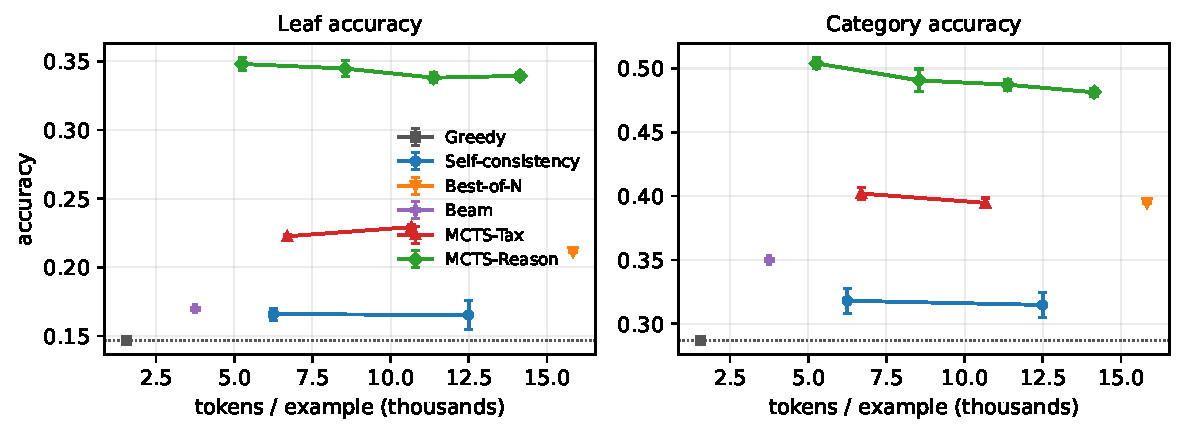
\includegraphics[width=\linewidth]{figures/budget_curve.pdf}
\caption{Accuracy vs.\ token budget (GPT-4.1-nano, $n{=}300$, mean $\pm$ std over
$5$ seeds; greedy, beam, and best-of-$N$ are single runs). $\mctsreas$ dominates
at every budget and is flat in its iteration knob; $\mctstax$ saturates between
$I{=}8$ and $I{=}16$; best-of-$N$ (reward, no tree) sits between
self-consistency and $\mctstax$; self-consistency barely improves on greedy.
What is searched matters far more than how much.}
\label{fig:budget}
\end{figure}
